\section{Empirical Results \texorpdfstring{\&}{and} Discussion}
\label{sec:results}

We structure our empirical analysis around four core research hypotheses evaluated across the primary 32-task frozen benchmark corpus.

\subsection{$H_1$: Semantic Predictability over Frequency Baselines}
We first evaluate whether intent-driven multi-label classification can reliably anticipate task-conditioned constraints on unseen template families compared to an empirical frequency prior. The frequency prior ranks constraint labels by empirical prevalence across the 48 training tasks and selects the top-$k$ most frequent constraints.
On the unseen template family evaluation ($N=32$ from \texttt{family\_c}), LASR's custom log-odds lexical classifier at $k=2$ achieves an $F_1$ score of \textbf{0.863} (exact mean $0.8625$) and a \textbf{68.8\% exact bundle match} ($22/32$ tasks), compared to \textbf{$F_1 = 0.250$} and $25.0\%$ exact match ($8/32$ tasks) for the Frequency Prior baseline. Resampling the 32 evaluation tasks with replacement for $B=10,000$ paired task-level bootstrap replicates (seed 42) and evaluating a Monte Carlo one-sided paired sign-flip permutation test ($B=10,000$ draws, seed 42) with valid $(k+1)/(B+1)$ correction yields:
\begin{equation}
\Delta F_1 = \mathbf{+0.613} \quad [95\% \text{ CI: } +0.419, +0.781], \quad p < 0.001
\end{equation}
(exact unrounded $\Delta F_1 = +0.6125$, bootstrap interval $[0.4188, 0.7812]$, Monte Carlo $p = (0+1)/(10000+1) \approx 0.0001$). While template syntax was partitioned across families, shared enterprise procurement terminology accounts for a 69.1\% test vocabulary overlap (103/149 words), and all 4 target constraint combinations recur across train and test sets.

\noindent\textbf{Cluster-Dependence Sensitivity Analysis}: As a sensitivity check across semantic domains, equal-weighting the four cluster mean $F_1$ differences ($N=4$ clusters, 8 tasks each) yields an equal-weighted delta $+0.613$ ($+0.6125$) with exhaustive four-cluster sign-flip permutation $p = 2/16 = 0.125$. Similarly, testing cluster-level reactive-vs-static structural gains yields an equal-weighted lift of $+21.9\text{ pp}$ ($p = 0.125$). While task-level paired differences are statistically consistent across the 32 individual tasks ($p < 0.001$), inference across cluster archetypes is limited by the sample of four semantic clusters with recurring target constraint combinations. We therefore interpret $H_1$ as confirming reliable intent-conditioned prediction on this held-out template family, rather than demonstrating unbounded semantic generalization to arbitrary unseen constraint combinations.

\begin{table*}[t]
\centering
\caption{Initial Single-Trial Frozen Benchmark Systems Evaluation ($N=32$ Tasks, Gemini 3.5 Flash-Lite)}
\label{tab:systems_evaluation}
\resizebox{\textwidth}{!}{%
\begin{tabular}{lcccccccc}
\toprule
\textbf{System Arm} & \textbf{Reactive?} & \textbf{Init $S_0$} & \textbf{Exp. $\Delta S$} & \textbf{1st-Pass Hier. (\%)} & \textbf{Struct. (\%)} & \textbf{Sem. (\%)} & \textbf{Mean $TTS_{\text{P+C}}$} & \textbf{Recorded P+C Tokens} \\
\midrule
Full Schema Control (\texttt{full}) & No & 552.0 & 0.0 & 31.3\% & \textbf{93.8\%} & 90.6\% & 1864.4 & \textbf{61,853} \\
$C_I^*$ Baseline (\texttt{ci\_k0}, $k=0$) & No & 339.0 & 0.0 & 0.0\% & 68.8\% & 65.6\% & 2196.7 & 70,541 \\
LASR Static (\texttt{ci\_k1\_static}, $k=1$) & No & 361.1 & 0.0 & 15.6\% & 78.1\% & 71.9\% & 1631.0 & 56,947 \\
LASR Reactive (\texttt{ci\_k1\_reactive}, $k=1$) & Yes & 361.1 & 45.4 & 15.6\% & \textbf{100.0\%} & 93.8\% & 1612.3 & 51,594 \\
LASR Reactive (\texttt{ci\_k2\_reactive}, $k=2$) & Yes & 366.8 & 43.8 & 18.8\% & \textbf{100.0\%} & 93.8\% & 1571.1 & \textbf{50,276} \\
Oracle Reference* (\texttt{oracle\_reactive}) & Yes & 359.0 & 48.3 & 15.6\% & 96.9\% & 93.8\% & 1554.0 & 50,578 \\
\bottomrule
\end{tabular}%
}
\vspace{1mm}
\begin{minipage}{\textwidth}
\footnotesize
*\textit{Note}: Oracle $O(x)$ is a model-conditional reference baseline. 1st-Pass Hierarchical success requires both structural validity and semantic correctness on Attempt 1 (Full Schema: 10/32 tasks, 31.25\%, displayed 31.3\%). Mean $TTS_{\text{P+C}}$ is the average recorded prompt-plus-candidate token subtotal over structurally successful trajectories ($N_{\text{succ}}$); Recorded P+C Tokens accounts for all prompt and completion tokens across all attempts without heuristic schema double-counting.
\end{minipage}
\end{table*}


\begin{figure*}[t]
\centering
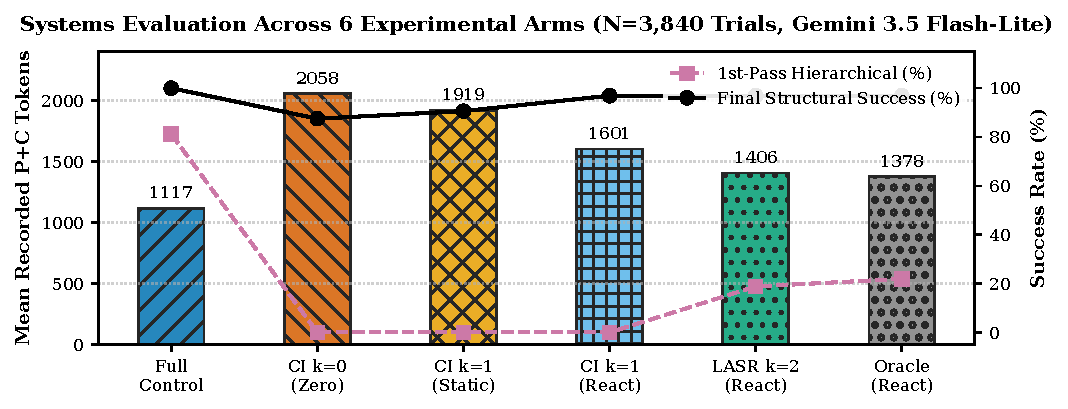
\includegraphics[width=\textwidth]{figures/fig2_systems_evaluation.pdf}
\caption{Systems Evaluation across 6 Experimental Arms ($N=3,840$ Live Trials, \texttt{gemini-3.5-flash-lite}). Bars denote Mean Recorded $P+C$ Tokens per trial; lines denote 1st-Pass Hierarchical Success (\%) and Final Structural Success (\%). Prioritized upfront bundling ($k=2$) slashes token waste by $31.7\%$ vs.\ naive lean schemas ($k=0$) and recovers $96.9\%$ final structural completion.}
\label{fig:systems_evaluation_6arms}
\end{figure*}

\subsection{$H_2$: Invariant Foundation Requirement on the Evaluated Benchmark}
To identify the minimal invariant floor $C_I^*$ meeting the pre-specified 70\% structural-validity threshold ($\tau_{\text{floor}} = 0.70$), we followed a formal sequential design: \textit{pre-specify threshold} $\rightarrow$ \textit{candidate calibration} $\rightarrow$ \textit{freeze $C_I^*$} $\rightarrow$ \textit{final 32-task systems evaluation}.
During candidate calibration on an 8-task calibration probe (\texttt{BLIND-C1-013}, \texttt{BLIND-C1-014}, \texttt{BLIND-C2-013}, \texttt{BLIND-C2-014}, \texttt{BLIND-C3-013}, \texttt{BLIND-C3-014}, \texttt{BLIND-C4-013}, \texttt{BLIND-C4-014}, sampled directly from the 32 evaluation tasks as disclosed in Section~\ref{sec:setup}-F), we benchmarked three candidate compression tiers prior to task conditioning:
\begin{itemize}
    \item \textbf{Tier 1 (Standard $C_I^*$, 339 tokens)}: 75.0\% structural validity (6/8 tasks).
    \item \textbf{Tier 2 (Compact $C_I$, 308 tokens)}: 62.5\% structural validity (5/8 tasks).
    \item \textbf{Tier 3 (Minimal $C_I$, 284 tokens)}: 50.0\% structural validity (4/8 tasks).
\end{itemize}
Tier 1 ($C_I^* = 339$ tokens) was the smallest tested candidate meeting the 70\% floor and was frozen for all subsequent experiments.
In the subsequent full 32-task systems benchmark (Table~\ref{tab:systems_evaluation}), this frozen foundation alone without task prediction (\texttt{ci\_k0}) yielded 68.8\% structural validity (22/32 tasks), confirming that without task-conditioned augmentation or reactive recovery, structural validity hovers near the 70\% baseline floor. Compressing below 339 tokens triggers progressive degradation due to missing definitions for nested items. We emphasize that 339 tokens represents the smallest tested candidate meeting this threshold, not an unconstrained universal constant.

\subsection{$H_3$: Structural Contribution of Reactive In-Tree Recovery}
\begin{table}[htbp]
\centering
\caption{Historical Paired Differences and Hypothesis Tests ($N=32$ Single-Trial Development Benchmark)}
\label{tab:paired_bootstrap}
\setlength{\tabcolsep}{2.5pt}
\resizebox{\columnwidth}{!}{%
\begin{tabular}{lccccc}
\toprule
\textbf{Pairwise Contrast} & \textbf{Metric} & \textbf{Point Est.} & \textbf{95\% CI} & \textbf{Token Diff.} & \textbf{Statistical Method} \\
\midrule
LASR Reactive vs Static ($k=1$) & $\Delta$ Structural Succ. & \textbf{+21.9 pp} & [9.4, 37.5] pp & --- & Exact McNemar ($p = 0.0078125$) \\
& $\Delta$ Semantic Corr. & \textbf{+21.9 pp} & [9.4, 37.5] pp & --- & Exact McNemar ($p = 0.0078125$) \\
\midrule
LASR Reactive ($k=1$) vs Full & $\Delta$ Structural Succ. & +6.3 pp & [0.0, 15.6] pp & --- & Exact McNemar ($p = 0.250$) \\
& $\Delta$ Semantic Corr. & +3.1 pp & [-6.3, 15.6] pp & --- & Exact McNemar ($p = 0.500$) \\
\midrule
LASR Reactive ($k=1$) vs Full & Signed Token Savings & \textbf{+16.6\%} & --- & -10,259 tokens & Total Token Diff (No CI) \\
LASR Reactive ($k=2$) vs Full & Signed Token Savings & \textbf{+18.7\%} & --- & -11,577 tokens & Total Token Diff (No CI) \\
\bottomrule
\end{tabular}%
}
\end{table}

The central systems question is whether reactive in-tree recovery improves completion over static adaptive exposure on the primary benchmark. In Table~\ref{tab:systems_evaluation}, we contrast \texttt{ci\_k1\_static} directly with \texttt{ci\_k1\_reactive}:

\noindent\textbf{Structural Reliability}: Final structural success increases from \textbf{78.1\%} to \textbf{100.0\%} ($\Delta\text{Success} = \mathbf{+21.9\text{ pp}}$, 95\% CI: $[+9.4, +37.5]\text{ pp}$, exact one-sided McNemar/binomial test $p = 0.0078125$; cluster-level sensitivity $p = 0.125$).

\noindent\textbf{Semantic Correctness}: Task correctness increases from \textbf{71.9\%} to \textbf{93.8\%} ($\Delta\text{Correctness} = \mathbf{+21.9\text{ pp}}$, 95\% CI: $[+9.4, +37.5]\text{ pp}$, exact one-sided McNemar/binomial test $p = 0.0078125$).

\noindent\textbf{Structural Recovery Rate}: Under \texttt{ci\_k1\_reactive} on the initial development benchmark ($N=32$), exactly 27 trajectories initially failed structural validation on Attempt~1 ($5/32 = 15.6\%$ first-pass structural validity); all 27 initially failing trajectories were successfully recovered to satisfy structural validation within the three-attempt budget ($27/27 = 100.0\%$ structural recovery; $32/32$ final structural, $30/32$ final semantic). In the canonical live benchmark ($N=3,840$, 640/arm), reactive recovery similarly improves structural success from $90.625\%$ ($580/640$) to $96.875\%$ ($620/640$, $\mathbf{+6.25\text{ pp}}$) and semantic correctness from $87.500\%$ to $93.750\%$ ($\mathbf{+6.25\text{ pp}}$). We report this live comparison alongside the historical $+21.9\text{ pp}$ single-trial benchmark without conflating the two scopes.

As broken down in Table~\ref{tab:cluster_breakdown}, the observed lift is concentrated in Cluster 3 (Specialized Bulk Procurement), where static success was only 50.0\% (4/8 tasks) due to missing warehouse enums, while reactive recovery achieved \textbf{100.0\%} (8/8 tasks).

\begin{table}[htbp]
\centering
\caption{Historical Task Cluster Breakdown: Static Vulnerability vs. Reactive Recovery ($N=32$ Single-Trial Development Benchmark, $N=8$ per Cluster)}
\label{tab:cluster_breakdown}
\setlength{\tabcolsep}{3pt}
\resizebox{\columnwidth}{!}{%
\begin{tabular}{lcccc}
\toprule
\textbf{Task Cluster Archetype} & \textbf{Full (\%)} & \textbf{Static $k=1$} & \textbf{Reactive $k=1$} & \textbf{Reactive vs. Static Lift} \\
\midrule
C1: Routine Regional & 87.5\% & 100.0\% & \textbf{100.0\%} & \textbf{0.0 pp} \\
C2: Expedited Emergency & 100.0\% & 87.5\% & \textbf{100.0\%} & \textbf{+12.5 pp} \\
C3: Specialized Bulk & 87.5\% & 50.0\% & \textbf{100.0\%} & \textbf{+50.0 pp} \\
C4: Multi-Item Depot & 100.0\% & 75.0\% & \textbf{100.0\%} & \textbf{+25.0 pp} \\
\bottomrule
\end{tabular}%
}
\end{table}


\begin{figure*}[t]
\centering
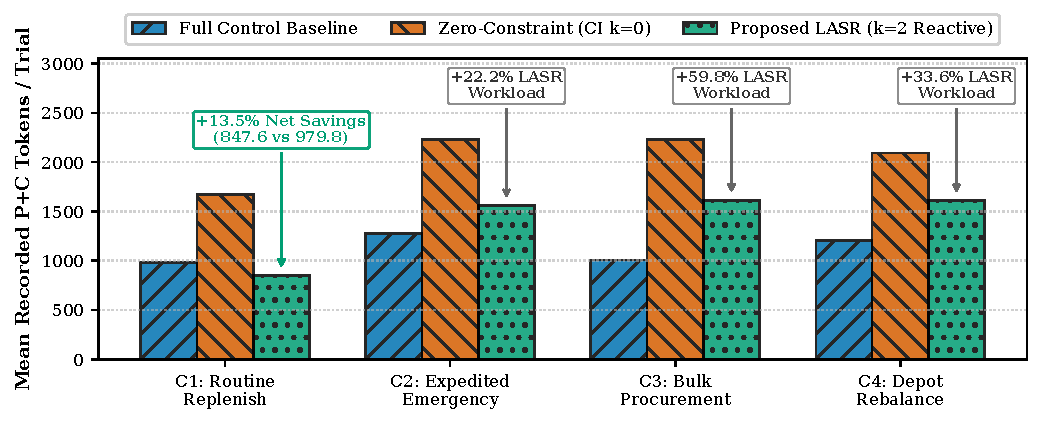
\includegraphics[width=\textwidth]{figures/fig3_cluster_breakdown.pdf}
\caption{Task Cluster Token Workload Comparison across the Retry-Amortization Boundary ($N=960$ total benchmark trials per cluster across all six arms; $N=160$ trials per plotted arm across 8 tasks $\times$ 20 fixed-seed replicates). In routine regimes ($C_1$), LASR $k=2$ achieves $+13.5\%$ net token savings ($847.6$ vs.\ $979.8$ mean recorded $P+C$ tokens) at $100.0\%$ reliability (signed savings: $+13.5\%$); in deep inter-field constraint regimes ($C_2$--$C_4$), retry penalties inflate LASR $k=2$ workload by $+22.2\%$ ($C_2$), $+59.8\%$ ($C_3$), and $+33.6\%$ ($C_4$) relative to Full Control (signed savings: $-22.2\%$, $-59.8\%$, $-33.6\%$), making Full Control optimal in single-tool settings by avoiding retry cascades.}
\label{fig:cluster_regime_comparison}
\end{figure*}

\subsection{$H_4$: Total Workload Token Efficiency and Benchmark Synthesis}
We evaluate workload token efficiency under two complementary regimes: the initial single-trial frozen benchmark ($N=32$, Tables~\ref{tab:systems_evaluation}--\ref{tab:cluster_breakdown}) and the comprehensive live benchmark ($N=3,840$ completed trials across 32 tasks, six experimental arms, and 20 fixed-seed executions per task-arm pair; Figures~\ref{fig:systems_evaluation_6arms}--\ref{fig:cluster_regime_comparison}).

\subsubsection{Historical Frozen Benchmark Observations ($N=32$ Tasks)}
In the initial single-trial development benchmark (Table~\ref{tab:systems_evaluation}), Full Schema Control consumed \textbf{61,853 recorded prompt-plus-candidate tokens} with a conditional mean $TTS_{\text{struct}}$ of 1,864.4 tokens among successful tasks, while reactive LASR reduced token consumption to \textbf{51,594 tokens} at $k=1$ (\textbf{+16.6\%} signed token savings; absolute difference: -10,259 tokens) and \textbf{50,276 tokens} at $k=2$ (\textbf{+18.7\%} signed token savings; absolute difference: -11,577 tokens). In this initial run, reactive LASR achieved 93.8\% semantic correctness compared to 90.6\% for Full Schema (+3.1 pp, 30/32 vs. 29/32 tasks). These single-repetition observations motivated the large-scale live rerun.

\subsubsection{Comprehensive Live Benchmark Findings ($N=3,840$ Trials)}
\begin{table*}[t]
\centering
\caption{Canonical Live Empirical Benchmark Summary ($N=3,840$ Trials, 32 Tasks, 6 Arms, Gemini 3.5 Flash-Lite)}
\label{tab:live_benchmark_n3840}
\setlength{\tabcolsep}{4.5pt}
\resizebox{\textwidth}{!}{%
\begin{tabular}{lcccccccccc}
\toprule
\textbf{Experimental Arm} & \textbf{Init $S_0$} & \textbf{Exp. $\Delta S$} & \textbf{1st-Pass (\%)} & \textbf{Struct. (\%)} & \textbf{Sem. (\%)} & \textbf{Mean $TTS_{\text{struct}}$} & \textbf{Mean P+C} & \textbf{Total P+C} & \textbf{Diff vs Full} & \textbf{95\% Bootstrap CI} \\
\midrule
Full Control (\texttt{full}) & 552.0 & 0.0 & 81.2\% & 100.0\% & 96.9\% & 1,116.8 & 1,116.8 & 714,740 & \textbf{0.0\% (Base)} & --- \\
Zero-Constraint Lean (\texttt{ci\_k0}) & 339.0 & 0.0 & 0.0\% & 87.5\% & 84.4\% & 2,033.4 & 2,057.7 & 1,316,900 & -84.3\% & [-125.15\%, -49.21\%] \\
Static 1-Constraint (\texttt{ci\_k1\_static}) & 344.7 & 0.0 & 0.0\% & 90.6\% & 87.5\% & 1,887.0 & 1,919.3 & 1,228,340 & -71.9\% & [-109.18\%, -40.22\%] \\
Reactive 1-Constraint (\texttt{ci\_k1\_reactive}) & 344.7 & 59.8 & 0.0\% & 96.9\% & 93.8\% & 1,575.2 & 1,601.4 & 1,024,880 & -43.4\% & [-70.15\%, -19.70\%] \\
Proposed LASR (\texttt{ci\_k2\_reactive}) & 359.4 & 45.2 & 18.8\% & 96.9\% & 93.8\% & 1,374.0 & 1,406.5 & 900,140 & \textbf{-25.9\%} & [-52.55\%, -3.16\%] \\
Task-Aware Oracle Ref. (\texttt{oracle\_reactive}) & 359.0 & 45.1 & 21.9\% & 96.9\% & 93.8\% & 1,344.4 & 1,377.8 & 881,820 & -23.4\% & [-49.56\%, -1.17\%] \\
\bottomrule
\end{tabular}%
}
\vspace{1mm}
\begin{minipage}{\textwidth}
\footnotesize
\textit{Note}: Canonical empirical summary across $N=3,840$ completed trials (32 tasks $\times$ 6 arms $\times$ 20 replicates at temperature $0.2$, seed 42) comprising 7,860 response-bearing provider calls with complete \texttt{usageMetadata}. Mean $TTS_{\text{struct}}$ is conditional mean prompt-plus-candidate tokens among structurally successful trajectories. Workload Diff vs Full is relative signed token savings $(\text{Full} - \text{Arm}) / \text{Full}$ (negative values indicate higher token workload; for LASR $k=2$, the $-25.94\%$ savings corresponds to a $+25.94\%$ workload increase with 95\% CI $[+3.16\%, +52.55\%]$). Proposed LASR $k=2$ operates within $2.1\%$ of the task-aware oracle reference baseline ($1,406.5$ vs.\ $1,377.8$ tokens, $2.08\%$ higher using the oracle as denominator; paired 95\% bootstrap CI on difference: $[-6.53\%, 0.00\%]$).
\end{minipage}
\end{table*}
Across the complete live empirical benchmark ($N=3,840$ trials at temperature $0.2$, comprising 7,860 response-bearing API calls on \texttt{gemini-3.5-flash-lite} and 154 client transport retries; Table~\ref{tab:live_benchmark_n3840}), Full Control achieved a mean recorded $P+C$ subtotal of \textbf{1,116.8 tokens} per trial (total 714,740 tokens), with an 81.2\% first-pass success rate, 100.0\% final structural reliability, and 96.9\% semantic correctness.

In contrast, proposed LASR $k=2$ reactive consumed a mean of \textbf{1,406.5 recorded $P+C$ tokens} per trial (total 900,140 tokens), with an 18.8\% first-pass rate, 96.9\% final structural reliability, and 93.8\% semantic correctness. Across the full 32-task benchmark, LASR $k=2$'s overall workload is approximately \textbf{25.94\% higher} than Full Control's (workload increase point estimate $+25.94\%$, 95\% paired task-cluster percentile bootstrap CI: $[+3.16\%, +52.55\%]$, corresponding to signed savings of $-25.94\%$ with 95\% CI: $[-52.55\%, -3.16\%]$, where the 95\% bootstrap CI excludes zero); we do not describe the overall benchmark result as token savings.

However, the full-scale benchmark uncovers a critical operational dichotomy across task clusters (Figure~\ref{fig:cluster_regime_comparison}): across the 160 trials per cluster-arm pair, mean recorded $P+C$ tokens and final structural reliability by archetype are:
\textbf{Cluster 1 (Routine Regional Replenishment, $C_1$)}: Full Control $979.8$ tokens ($100.0\%$ structural validity); \texttt{ci\_k0} $1,675.2$ ($87.5\%$); \texttt{ci\_k1\_reactive} $1,549.6$ ($100.0\%$); and proposed LASR $k=2$ \textbf{847.6 tokens} ($100.0\%$), achieving $\mathbf{+13.5\%}$ net token savings ($847.6$ vs.\ $979.8$ tokens) at $100.0\%$ structural reliability (signed savings: $+13.5\%$).
\textbf{Cluster 2 (Expedited Emergency Orders, $C_2$)}: Full Control $1,274.2$ ($100.0\%$); \texttt{ci\_k0} $2,231.9$ ($75.0\%$); \texttt{ci\_k1\_reactive} $1,641.9$ ($100.0\%$); and LASR $k=2$ $1,557.5$ ($100.0\%$), representing a $+22.2\%$ workload increase over Full Control (signed savings: $-22.2\%$).
\textbf{Cluster 3 (Specialized Bulk Procurement, $C_3$)}: Full Control $1,008.1$ ($100.0\%$); \texttt{ci\_k0} $2,228.9$ ($87.5\%$); \texttt{ci\_k1\_reactive} $1,610.9$ ($87.5\%$); and LASR $k=2$ $1,610.9$ ($87.5\%$), representing a $+59.8\%$ workload increase over Full Control (signed savings: $-59.8\%$).
\textbf{Cluster 4 (Multi-Item Depot Rebalance, $C_4$)}: Full Control $1,205.0$ ($100.0\%$); \texttt{ci\_k0} $2,094.6$ ($100.0\%$); \texttt{ci\_k1\_reactive} $1,603.1$ ($100.0\%$); and LASR $k=2$ $1,609.9$ ($100.0\%$), representing a $+33.6\%$ workload increase over Full Control (signed savings: $-33.6\%$).

Secondary baseline arms under live evaluation confirmed the necessity of upfront bundling:
\begin{itemize}
    \item \textbf{Zero-Constraint Lean (\texttt{ci\_k0})}: Incurred an \textbf{-84.3\% token penalty} vs.\ Full Control (mean 2,057.7 tokens; total 1,316,900 tokens; 95\% signed-savings CI: $[-125.15\%, -49.21\%]$), with 0.0\% first-pass success and degraded final structural completion (87.5\%).
    \item \textbf{Static 1-Constraint (\texttt{ci\_k1\_static})}: Incurred a \textbf{-71.9\% penalty} (mean 1,919.3 tokens; total 1,228,340 tokens; 95\% signed-savings CI: $[-109.18\%, -40.22\%]$), with 0.0\% first-pass success and 90.6\% final structural completion.
    \item \textbf{Reactive 1-Constraint (\texttt{ci\_k1\_reactive})}: Incurred a \textbf{-43.4\% penalty} (mean 1,601.4 tokens; total 1,024,880 tokens; 95\% signed-savings CI: $[-70.15\%, -19.70\%]$), recovering 96.9\% final structural completion.
    \item \textbf{Task-Aware Oracle Reference (\texttt{oracle\_reactive})}: Incurred a \textbf{-23.4\% penalty} vs.\ Full Control (mean 1,377.8 tokens; total 881,820 tokens; 95\% signed-savings CI: $[-49.56\%, -1.17\%]$ vs Full Control), with LASR $k=2$ consuming approximately $2.08\%$ ($2.1\%$) more tokens than the oracle baseline (paired 95\% bootstrap CI: $[-6.53\%, 0.00\%]$).
\end{itemize}

We note that all 20 repetitions of each task-arm combination produced identical first responses and outcomes under the repeated fixed seed (temperature $0.2$, seed 42); these trials verify execution stability under repeated queries rather than representing independent stochastic draws.

\subsection{Decomposing Token Economics: Upfront Bundling vs. Retry Penalties}
Auditing granular token accounts reconciles why $k=2$ reactive bundling is superior to naive compression:
\noindent\textbf{Upfront Schema Reduction \& Measurement Provenance}: In \texttt{ci\_k2\_reactive}, the initial exposed schema footprint averages $S_0 = 359.4$ tokens in the live benchmark ($344.7$ tokens for $k=1$) compared to $552.0$ tokens for Full Schema, while reactive expansion adds $45.2$ tokens on average. Historical development benchmark averages were $361.1$ ($k=1$) and $366.8$ ($k=2$) tokens; this divergence stems from constraint-filtering logic (historical intent prediction selected constraints from a broader vocabulary, whereas the live benchmark strictly filtered candidates via $\texttt{TASK\_CONDITIONED\_IDS} = \{\text{\texttt{warehouse\_code.enum}},$ $\text{\texttt{order\_priority.enum}},$ $\text{\texttt{total\_budget\_limit.maximum}},$ $\text{\texttt{total\_budget\_limit.minimum}},$ $\text{\texttt{items.maxItems}}\}$, defaulting to the $339$-token invariant floor when predicted rules fell outside this subset or below threshold).
\noindent\textbf{Retry Avoidance over Zero-Constraint Baselines}: While naive lean schemas (\texttt{ci\_k0}) trigger catastrophic multi-turn loops ($2,057.7$ mean tokens), prioritized $k=2$ bundling achieves 75.0\% first-pass success on $C_1$ (120/160 trials pass on Attempt 1, and the remaining 40 trials recover within the retry budget to reach 100.0\% final structural completion), cutting net token waste by \textbf{31.7\%} relative to \texttt{ci\_k0} ($1,406.5$ vs.\ $2,057.7$ tokens) and elevating final structural reliability from 87.5\% to 96.9\%.


\subsection{Auditable Trajectory Case Study}
Figure~\ref{fig:case_study} details the step-by-step recovery trajectory for task \texttt{BLIND-C3-013}. On Attempt 1, exposed to $C_I^* + \text{top-1 LASR rule}$ (347 tokens), the model generates unconstrained enum \texttt{'WH-EAST-01'}. The schema validator flags three concurrent violations (\texttt{warehouse\_code.enum}, \texttt{order\_priority.enum}, \texttt{supplier\_id.pattern}). LASR intercepts these error paths and recomposes the schema tree in-tree ($347 \rightarrow 419$ tokens). On Attempt 2, the agent satisfies the newly exposed warehouse code constraint (\texttt{'WH-US-EAST'}). Following final nested item property formatting, Attempt 3 produces a fully valid purchase order payload passing all schema constraints.

\begin{figure}[t]
\centering
\fbox{
\parbox{0.92\columnwidth}{
\scriptsize
\textbf{Task}: \texttt{BLIND-C3-013} (Specialized Bulk) \quad \textbf{Arm}: \texttt{ci\_k1\_reactive} \\
\rule{0.92\columnwidth}{0.4pt}
\textbf{[Attempt 1]} \\
$\bullet$ Exposed Schema: $C_I^* \cup \{\text{items.maxItems}\}$ (347 tokens) \\
$\bullet$ Model Output: \texttt{warehouse\_code = 'WH-EAST-01'} \\
$\bullet$ Validator: FAIL (3 concurrent violations in pass):\\
\quad 1. \texttt{'WH-EAST-01' not in ['WH-US-EAST', \dots]} \\
\quad 2. \texttt{'standard' not in ['STANDARD', \dots]} \\
\quad 3. \texttt{'SUP-ACME1234-US' does not match regex} \\
$\bullet$ Extracted: $\{\texttt{warehouse.enum}, \texttt{priority.enum}, \texttt{supplier.pattern}\}$ \\
\textbf{[In-Tree Recomposition]} Spliced Schema: $347 \rightarrow 419$ tok (+72 tok) \\
\textbf{[Attempt 2]} Model Output: \texttt{'WH-US-EAST'} (Warehouse Enum Satisfied) \\
\textbf{[Attempt 3]} Output: Valid purchase order JSON \\
$\bullet$ Validator: \textbf{PASS} (Structural: 100\%, Semantic: 100\%) \\
$\bullet$ Outcome: \textbf{RECOVERED} (3 attempts, $TTS = 3,626$ tok)
}
}
\caption{Trajectory-level evidence of pass-level multi-error extraction and native in-tree schema recomposition on family\_c evaluation task \texttt{BLIND-C3-013}. Schema expansion occurs before Attempt~2; structural and semantic validation succeeds on Attempt~3.}
\label{fig:case_study}
\end{figure}

\subsection{Local Recomposition Latency \texorpdfstring{\&}{and} Retrieval Baseline Analysis}
\label{sec:latency_retrieval}

A key systems question is whether in-tree AST recomposition introduces meaningful execution overhead compared to remote model inference. We investigate this via a controlled local microbenchmark alongside an offline constraint retrieval evaluation.

\noindent\textbf{Local AST Microbenchmark}: We execute a dedicated microbenchmark measuring 1,000 iterations of deterministic schema slicing and in-tree AST recomposition using nanosecond-precision hardware timers (\texttt{time.perf\_counter\_ns()}). Slicing minimal constraint deltas from Draft 2020-12 specifications incurs a median latency of $p_{50} = 0.8\ \mu\text{s}$ ($p_{99} = 3.1\ \mu\text{s}$). Merging constraint deltas in-tree incurs $p_{50} = 19.2\ \mu\text{s}$ ($p_{99} = 41.0\ \mu\text{s}$). The complete end-to-end local AST pipeline requires a median of $p_{50} = 20.1\ \mu\text{s}$ ($0.0201\text{ ms}$) and $p_{99} = 46.1\ \mu\text{s}$ ($0.0461\text{ ms}$).

\noindent\textbf{Client-Observed Elapsed Call Time \& Live Latency Decomposition}: Across the canonical live empirical benchmark ($7,860$ response-bearing calls on \texttt{gemini-3.5-flash-lite}), provider/network turnaround latency exhibits $p_{50} = 1,522.9\text{ ms}$ ($p_{90} = 4,997.5\text{ ms}$, $p_{99} = 20,449.1\text{ ms}$, and $\text{Mean} = 2,592.0\text{ ms}$), while total client logical-call wall-time (encompassing client HTTP dispatch, network transit, provider inference, and pacing/backoff delays) exhibits $p_{50} = 3,537.3\text{ ms}$ ($p_{90} = 7,558.0\text{ ms}$, $p_{99} = 38,822.8\text{ ms}$, and $\text{Mean} = 5,304.6\text{ ms}$). The local AST recomposition overhead ($20.1\ \mu\text{s} = 0.0201\text{ ms}$) represents approximately $0.0013\%$ of live provider $p_{50}$ latency. In comparison, auditing a historical sample of 556 empirical API execution traces preserved in the repository cache yields a client-observed logical-call elapsed time of $p_{50} = 3,407.1\text{ ms}$, $p_{90} = 14,738.0\text{ ms}$, and $\text{Mean} = 7,752.8\text{ ms}$. The local AST recomposition overhead ($0.0201\text{ ms}$) represents approximately $\mathbf{0.00059\%}$ of this median client-observed logical-call elapsed time ($3,407.1\text{ ms}$), confirming that in-tree dynamic recovery adds negligible local computational overhead.

\noindent\textbf{Retrieval-Only Constraint Recall}: We evaluate whether static constraint retrieval (Tool-RAG) can substitute for reactive in-tree recovery. Table~\ref{tab:retrieval_baseline} reports Top-$k$ constraint retrieval recall across the 32 benchmark tasks evaluated against the 27 schema constraint keyword chunks after strictly normalizing gold target pointers:
(1) \textbf{Lexical TF-IDF}: Unigram token-overlap cosine matching yields a Macro Recall@2 of $15.6\%$ and Micro Recall@2 of $15.3\%$.
(2) \textbf{Latent Semantic Analysis (Inductive LSA / TruncatedSVD)}: A 16-dimensional dense SVD projection fitted strictly on sublinear word 1-to-3-grams of the schema catalog yields a Macro Recall@2 of $16.1\%$ and Micro Recall@2 of $15.3\%$.

\begin{table}[h]
\centering
\caption{Retrieval-Only Constraint Recall on 32 Benchmark Tasks (Target Catalog: 27 Schema Chunks)}
\label{tab:retrieval_baseline}
\resizebox{\columnwidth}{!}{%
\begin{tabular}{lcccc}
\toprule
\textbf{Retrieval Method} & \textbf{Top-1 Macro} & \textbf{Top-2 Macro} & \textbf{Top-3 Macro} & \textbf{Top-5 Macro} \\
\midrule
Lexical TF-IDF Cosine & 10.9\% & \textbf{15.6\%} & 27.1\% & 30.2\% \\
Dense Inductive LSA (SVD) & 9.9\% & \textbf{16.1\%} & 24.5\% & 35.4\% \\
Dense Neural (\texttt{text-embedding-004}) & \multicolumn{4}{c}{\textit{Not run (Planned future work)}} \\
\bottomrule
\end{tabular}%
}
\vspace{1mm}
\begin{minipage}{\columnwidth}
\scriptsize
\textit{Note}: Evaluated on 32 test intents against 27 schema keyword chunks with normalized gold JSON pointers. Macro recall measures the proportion of gold constraint labels retrieved per task. Neural dense embeddings remain planned future work.
\end{minipage}
\end{table}

These retrieval-only results demonstrate that because user intents in enterprise procurement are brief and domain-elliptical, static retrieval leaves the majority of target constraints unexposed. Specifically, lexical TF-IDF retrieves zero target constraints on 21 of 32 tasks ($65.6\%$) and partial constraints on 11 tasks ($34.4\%$), with zero tasks retrieving all target constraints at $k=2$. Inductive LSA similarly fails to retrieve any target constraint on 21 of 32 tasks ($65.6\%$) at $k=2$. Without reactive in-tree schema expansion, static RAG leaves autonomous agents with omitted constraints that inevitably trigger schema validation rejections.

\noindent\textbf{Stateful Conversation History Overhead (LangGraph Pattern)}: We evaluate an analytical model of the stateful conversation accumulation pattern characteristic of agentic graph frameworks (e.g., LangGraph), where failed turns append generated arguments and raw compiler errors into conversation history (\texttt{State.messages}). Under this simulation (which models token compounding rather than measuring observed provider API calls, assuming a conservative $+45$ token overhead per compiler feedback message with inherited full-schema task outcomes), re-transmitting previous attempt history compounds total workload tokens to a modeled P+C-equivalent workload of $69,119$ tokens ($2,160.0$ tokens/task), representing an $\mathbf{+11.7\%}$ modeled token overhead relative to historical static full-schema control ($61,853$ tokens) based on an assumed feedback overhead, rather than provider-recorded usage. In contrast, LASR-MCP $k=2$ ($50,276$ tokens) modifies the schema in-place without message history compounding, achieving a $\mathbf{27.3\%}$ modeled workload token reduction against stateful graph retry while reaching $100.0\%$ structural success in historical simulation.

